\section{Geometric Transformations}
Il processo che va dagli oggetti tridimensionali alle scene sintetiche bidimensionali coinvolge una sequenza di trasformazioni da uno spazio all'altro. A sua volta, questa sequenza richiede la definizione e il calcolo di adeguate trasformazioni.
L'\textbf{object space} è il riferimento in cui si definisce un modello 3D (ad esempio, lo spazio in cui si definiscono le coordinate dei punti, le normali, ...). Ogni oggetto 3D ha il suo spazio, scelto arbitrariamente dal modellatore (ci sono convenzioni).
Una scena è di solito composta da diversi oggetti. Il \textbf{world space} è il sistema di riferimento comune alla scena.
Abbiamo bisogno di una mappa dall'object space al world space: la \textbf{trasformazione di modellazione}.
\begin{figure}[H]
    \centering
    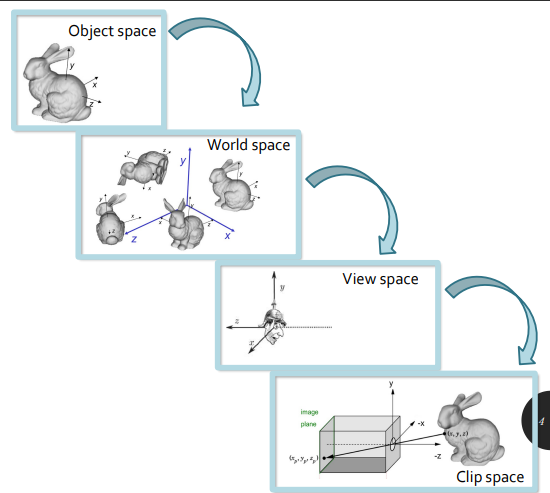
\includegraphics[width=0.5\textwidth]{images/SpaceObject.png} 
    \caption{Geometric Transformations}
    \label{fig:immagine}
\end{figure}
La trasformazione di modellazione riflette come ogni modello è posizionato nella scena. Ogni oggetto 3D ha la propria trasformazione di modellazione. Le trasformazioni includono, ad esempio, rotazioni degli oggetti, traslazioni e scalature. Queste trasformazioni affini sono rappresentate come matrici.
Il \textbf{view space} (spazio della fotocamera, spazio dell'occhio) ha l'origine nel centro della fotocamera. Abbiamo bisogno di una seconda trasformazione dallo spazio del mondo allo spazio di vista.
Nota: le trasformazioni possono essere composte in una singola trasformazione (da oggetto a vista).Lo spazio di clip è lo spazio finale di destinazione, allineato con lo schermo bidimensionale del dispositivo di output. Il mapping dallo spazio di vista allo \textbf{spazio di clip} coinvolge la proiezione degli elementi tridimensionali sul piano bidimensionale. Le proiezioni non sono trasformazioni affini.
Messaggio chiave: Se vogliamo passare dalla geometria tridimensionale allo schermo, abbiamo bisogno di trasformazioni che agiscano su punti e vettori.
\subsection{Recap: Point and Vectors}
Le entità fondamentali nella Grafica Computazionale sono i \textbf{punti} (cioè, le posizioni) e i \textbf{vettori} (cioè, gli spostamenti, le direzioni). Anche se hanno rappresentazioni simili nello spazio tridimensionale (cioè, triplette di coordinate), il loro significato geometrico e fisico è completamente diverso. Operazioni diverse hanno senso per entità diverse.
\begin{align*}
\text{point - point} & = \text{vettore (spostamento)} \\
\text{point + vector} & = \text{punto (traslato)} \\
\text{vector + vector} & = \text{vettore (legge del parallelogramma)} \\
\text{vector - vector} & = \text{vettore (legge del parallelogramma)} \\
\text{scalare} \cdot \text{vettore} & = \text{vettore (magnitudine e lunghezza scalate)}
\end{align*}
\begin{figure}[H]
    \centering
    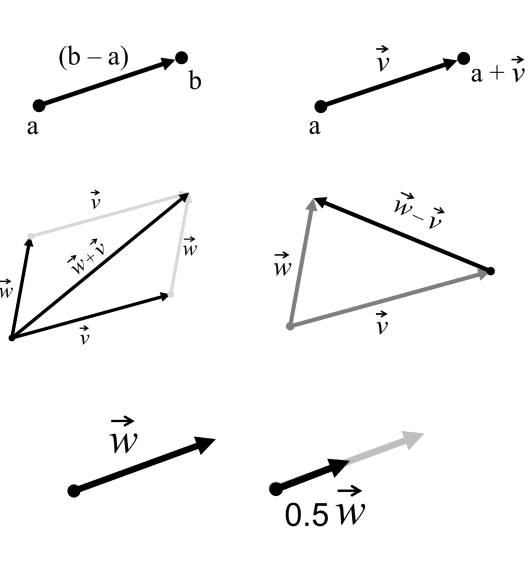
\includegraphics[width=0.5\textwidth]{images/PointVec.png} 
    \caption{Punti e Vettori}
    \label{fig:immagine}
\end{figure}
\textbf{Prodotto scalare}: da due vettori a uno scalare (somma dei prodotti delle coordinate corrispondenti)  
\textbf{Prodotto vettoriale}: da due vettori a un vettore, ortogonale ad entrambi i vettori di partenza (in \(\mathbb{R}^3\)); l'orientamento dipende dall'ordine degli operandi.
\subsection{Affine transformations 2D}
Le trasformazioni affini includono \textbf{traslazione, rotazione, scalatura, scorrimento e riflessione}. La composizione delle trasformazioni affini è una trasformazione affine.
\subsubsection{Translation(2D)}
Traslare un oggetto geometrico nel piano 2D implica spostare ciascun punto P dell'oggetto lungo l'asse x e l'asse y, tramite due quantità scalari (ricordando l'algebra dei punti e dei vettori: 
è possibile sommare un punto e un vettore e ottenere...).

\subsubsection{Scaling(2D)}
Rispetto a un punto fisso, qui si assume che il punto sia l'origine del riferimento.
Ridimensionare un punto P significa posizionare P ad una nuova distanza dagli assi; ridimensionare un oggetto significa ridimensionare tutti i suoi punti. Effetto: cambiano le dimensioni lungo gli assi (confronta gli effetti dei fattori di ridimensionamento maggiori o minori di 1).
Nota: moltiplicazione di matrici.
\subsubsection{Rotation(2D)}
Attorno a un punto fisso
Presupposti: centro di rotazione nell'origine del sistema di riferimento
Ruotare un punto P significa spostare P attorno al punto fisso per un certo angolo; ancora una volta, ruotare un oggetto significa ruotare solidamente tutti i suoi punti.
Angoli positivi implicano direzione antioraria, angoli negativi direzione oraria.
Nota: moltiplicazione di matrici.
Le formule possono essere calcolate utilizzando l'espressione di P nelle coordinate polari.
\subsubsection{Composing Transformations}
Le formule che abbiamo visto per la rotazione e la scalatura assumono che il punto fisso sia lo stesso dell'origine del sistema di riferimento. Come possiamo fare per ruotare (o ridimensionare) rispetto a un punto che non è l'origine del sistema di riferimento?
Idea di composizione delle trasformazioni:
\begin{itemize}
\item Applicare una traslazione per spostare l'origine al punto dato
\item Ruotare (o scalare)
\item Applicare la traslazione inversa per riportare l'origine
\end{itemize}

Possiamo farlo con una singola matrice?
\textbf{Problema}:
\begin{itemize}
\item La traslazione è espressa come una somma
\item La rotazione (o scalatura) è espressa come un prodotto
\end{itemize}

\textbf{Soluzione}:
\begin{itemize}
\item Coordinate omogenee: una rappresentazione diversa per punti e vettori (non più coordinate cartesiane)
\end{itemize}
\subsubsection{Homogeneous coordinates (2D)}
Un punto P le cui coordinate cartesiane sono (x, y) viene rappresentato con \textit{coordinate omogenee}.
$(x_h,y_h,w), w \neq 0  $
$x=x_h/w; y=y_h/w  $
Due triple rappresentano lo stesso punto se una è un multiplo dell'altra.
Poiché w non è zero, possiamo adottare la \textbf{forma canonica} come rappresentante della classe di coordinate omogenee che rappresentano lo stesso punto.
$(x,y,w) -> (x/w,y/w,1)$
Vantaggio: le coordinate omogenee eliminano l'ambiguità tra punti (posizioni) e vettori (direzioni).
Le terne con 1 come terza coordinata sono punti, mentre le terne con 0 come terza coordinata possono essere viste come punti all'infinito, quindi direzioni (torneremo su questo argomento).
\subsubsection{Translation revisited (2D)}
Nota: poiché ora abbiamo tre coordinate per punti e vettori, avremo matrici di dimensione 3 per 3. È facile verificare che la concatenazione delle traslazioni mediante moltiplicazione dà una traslazione per una quantità lungo ciascun asse che è la somma delle singole quantità.
\begin{figure}[H]
    \centering
    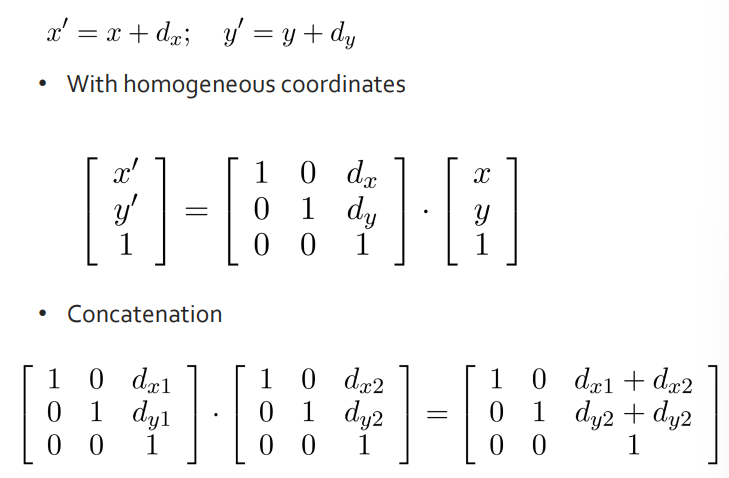
\includegraphics[width=0.5\textwidth]{images/CoorddinNonRic.png} 
    \caption{Punti e Vettori}
    \label{fig:immagine}
\end{figure}
\subsubsection{Scaling revisited (2D)}
Rispetto a un punto fisso
Ancora una volta, concatenazione tramite moltiplicazione di matrici.
\\
$x'=x+d_x;y'=y+d_y$
\\
$\begin{bmatrix}
    x' \\
    y' \\
    1 \\
\end{bmatrix}
=
\begin{bmatrix}
1 & 0 & d_x \\
0 & 1 & d_y \\
0 & 0 & 1\\
\end{bmatrix}
*
\begin{bmatrix}
    x \\
    y \\
    1 \\
\end{bmatrix}
$
\\
\textbf{Concatenation}
\\
$
\begin{bmatrix}
    1 & 0 & d_x1 \\
    0 & 1 & d_y1 \\
    0 & 0 & 1 \\
\end{bmatrix}
*
\begin{bmatrix}
    1 & 0 & d_x2 \\
    0 & 1 & d_y2 \\
    0 & 0 & 1 \\
\end{bmatrix}
=
\begin{bmatrix}
    1 & 0 & d_x1+d_x2 \\
    0 & 1 & d_y1+d_y2 \\
    0 & 0 & 1 \\
\end{bmatrix}
$
\subsubsection{Scaling Revisited}
Rispetto a un punto fisso, ancora una volta, concatenazione tramite moltiplicazione di matrici.
\\
$x'=s_x*x; y'=s_y*y$
\\
With omogeneous coordinates \\

$x'=x+d_x;y'=y+d_y$
\\
$\begin{bmatrix}
    x' \\
    y' \\
    1 \\
\end{bmatrix}
=
\begin{bmatrix}
s_x & 0 & 0 \\
0 & s_y & 0 \\
0 & 0 & 1 \\
\end{bmatrix}
*
\begin{bmatrix}
    x \\
    y \\
    1 \\
\end{bmatrix}
$
\\
$
\begin{bmatrix}
s_x1 & 0 & 0 \\
0 & s_y1 & 0 \\
0 & 0 & 1 \\
\end{bmatrix}
*
\begin{bmatrix}
    s_x2 & 0 & 0 \\
    0 & s_y2 & 0 \\
    0 & 0 & 1 \\
\end{bmatrix}
=
\begin{bmatrix}
    s_x1*s_x2 & 0 & 0 \\
    0 & s_y1*s_y2 & 0 \\
    0 & 0 & 1 \\
\end{bmatrix}
$ \\
Scaling attorno ad un \textbf{punto arbitrario} $P=(P_x,P_y)$ \\
$S_g=
    \begin{bmatrix}
    1 & 0 & P_x \\
    0 & 1 & P_y \\
    0 & 0 & 1 \\
    \end{bmatrix}
    *
    \begin{bmatrix}
        s_x & 0 & 0 \\
       0 & s_y & 0 \\
        0 & 0 & 1 \\
    \end{bmatrix}
    *
    \begin{bmatrix}
        1 & 0 & -P_x \\
        0 & 1 & -P_y \\
        0 & 0 & 1 \\
    \end{bmatrix} $
\subsubsection{Rotation revisited (2D)}
Intorno a un punto fisso, con il centro di rotazione nell'origine del sistema di riferimento.
$x'=x*cos\theta-y*sin \theta; y'=x*sin \theta + y*cos\theta$ \\
Con coordinate omogenee:
\\
$\begin{bmatrix}
    x' \\
    y' \\
    1 \\
\end{bmatrix}
=
\begin{bmatrix}
cos \theta & -sin \theta & 0 \\
sin \theta & cos \theta & 0 \\
0 & 0 & 1 \\
\end{bmatrix}
*
\begin{bmatrix}
    x \\
    y \\
    1 \\
\end{bmatrix}
$
\\
Rotazione attorno ad un punto arbitrario $P = (Px,Py)$ \\
$R_g=
    \begin{bmatrix}
    1 & 0 & P_x \\
    0 & 1 & P_y \\
    0 & 0 & 1 \\
    \end{bmatrix}
    *
    \begin{bmatrix}
        cos \theta & -sin \theta & 0 \\
        sin \theta & cos \theta & 0 \\
        0 & 0 & 1 \\
    \end{bmatrix}
    *
    \begin{bmatrix}
        1 & 0 & -P_x \\
        0 & 1 & -P_y \\
        0 & 0 & 1 \\
    \end{bmatrix} $
\subsubsection{Riassumendo}
Dalle coordinate cartesiane alle coordinate omogenee
• Possiamo rappresentare in modo univoco le trasformazioni come matrici, e possiamo facilmente comporre trasformazioni dello stesso tipo
• Torniamo al nostro problema di comporre trasformazioni di tipi diversi
• La buona notizia è che con le coordinate omogenee, ogni sequenza di trasformazioni si riduce all'applicazione di una singola matrice, che è il prodotto delle singole matrici che rappresentano le trasformazioni (ricorda che questo non era il caso con le coordinate cartesiane)
\subsubsection{Concatenation of transformations} 
Nota: l'ordine è importante! La moltiplicazione tra matrici in generale non è commutativa. Esempio: il bianco è l'input, il grigio scuro è il risultato. A sinistra: prima rotazione, poi scalatura; A destra: prima scalatura, poi rotazione.
\begin{figure}[H]
    \centering
    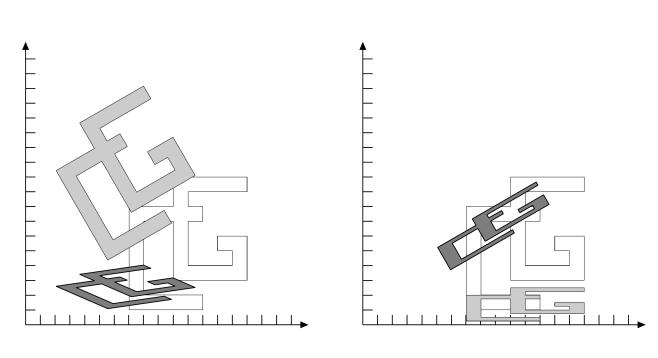
\includegraphics[width=0.5\textwidth]{images/ConcTransf.png} 
    \caption{Concatenation of Transformations}
    \label{fig:immagine}
\end{figure}
Per mappare dallo spazio dell'oggetto allo spazio del mondo, è possibile concatenare trasformazioni affini e rappresentare la concatenazione con una singola matrice, utilizzando coordinate omogenee. Attraverso la moltiplicazione delle matrici, si otterranno le coordinate nello spazio del mondo. Allo stesso modo, le composizioni vengono utilizzate per propagare le trasformazioni lungo i nodi dei grafi della scena.
\subsubsection{Reflection (2D)}
\begin{figure}[H]
    \centering
    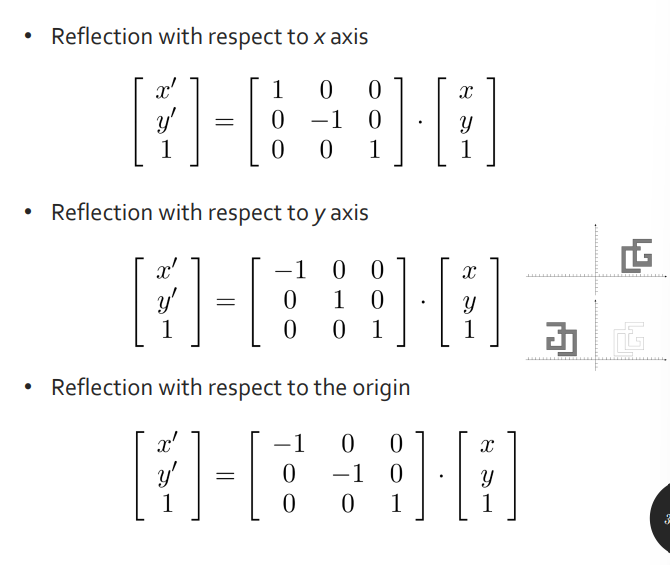
\includegraphics[width=0.5\textwidth]{images/Reflection.png} 
    \caption{Reflection(2D)}
    \label{fig:immagine}
\end{figure}
\subsubsection{Shear (2D)}
La quantità di deformazione di un punto lungo l'asse x dipende dalla coordinata y del punto, e viceversa.
\begin{figure}[H]
    \centering
    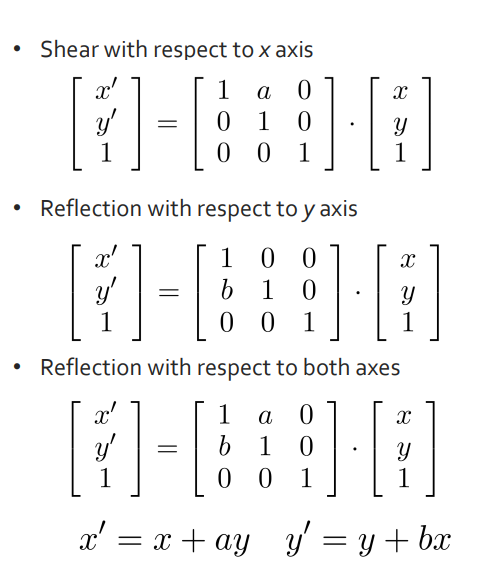
\includegraphics[width=0.5\textwidth]{images/Shear.png} 
    \caption{Reflection(2D)}
    \label{fig:immagine}
\end{figure}
\subsection{Affine transformations 3D}
Si possono utilizzare le coordinate omogenee anche in tre diemnsioni.
$p=\begin{bmatrix}
    x \\
    y \\
    z \\
    1 \\
\end{bmatrix}
$ \\
$v=\begin{bmatrix}
    x \\
    y \\
    z \\
    0 \\
\end{bmatrix}
$
In questo caso abbiamo tre assi utilizzati per deinire l'orientamento.
Esempio di coordinate omogenee:
\\
$T(d_x,d_y,d_z)=
\begin{bmatrix}
    1 & 0 & 0 & d_x \\
    1 & 0 & 0 & d_y \\
    1 & 0 & 0 & d_z \\
    1 & 0 & 0 & 1 \\
\end{bmatrix}$
\subsubsection{Rotation(3D)}
Abbiamo bisogno di identificare l'angolo, la direzione e l'asse. Le rotazioni intorno agli assi cartesiani possono essere facilmente derivate dal caso 2D. Le rotazioni intorno ad assi arbitrari possono essere ottenute componendo traslazioni + rotazioni intorno agli assi cartesiani.
\begin{figure}[H]
    \centering
    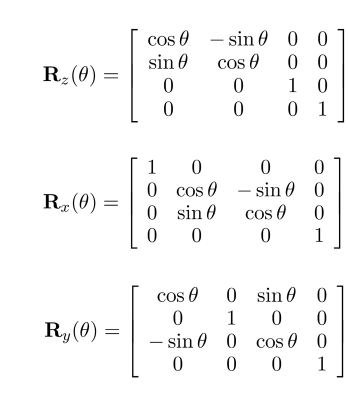
\includegraphics[width=0.5\textwidth]{images/Rot3D.png} 
    \caption{Rotation Matrix (3D)}
    \label{fig:immagine}
\end{figure}
\subsubsection{Recap from the rendering pipeline}
Descriviamo la relazione tra l'osservatore e la fotocamera attraverso la metafora della fotocamera a foro stenopeico. Abbiamo un foro infinitamente piccolo, l'immagine si forma sul piano sul retro della fotocamera, mentre assumiamo di avere anche un piano virtuale ad una distanza d dal centro di proiezione, dove d è la lunghezza focale.
Problema: come derivare le coordinate 2D sull'immagine delle entità nella scena 3D.
Abbiamo diverse scelte, in base al tipo di informazione che si desidera rappresentare.
\subsubsection{Prospective and Parallel projections}
Le proiezioni sono definite da una serie di linee rette, chiamate proiettori, che hanno un'origine comune nel centro di proiezione. Attraversano i punti della primitiva 3D e intersecano il piano di proiezione per formare la proiezione. Poiché la proiezione di un segmento è un segmento, proiettare i vertici è sufficiente. Se i proiettori sono linee rette e il piano di proiezione è effettivamente un piano, parliamo di proiezioni planari.
\textbf{Proiezioni prospettiche}: il centro ha una distanza finita dal piano.
\textbf{Proiezioni parallele}: la distanza non è finita e i proiettori sono linee parallele.
Effetto fisheye vs preservare le proporzioni.
\begin{figure}[H]
    \centering
    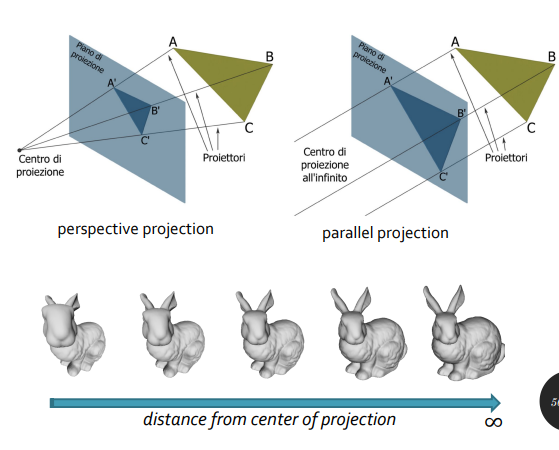
\includegraphics[width=0.5\textwidth]{images/ProspParall.png} 
    \caption{Prospective and Parallel}
    \label{fig:immagine}
\end{figure}
Le proiezioni prospettiche sono realistiche. Tuttavia, le distanze non vengono preservate e le linee parallele non sono più parallele.
Con le proiezioni parallele, invece, la vista può essere meno realistica, ma le distanze vengono preservate così come il parallelismo, quindi sono utili se si devono effettuare misurazioni.

Proiezioni ortografiche parallele: il piano dell'immagine è perpendicolare a uno degli assi del sistema cartesiano, che identifica la direzione di proiezione.
\begin{figure}[H]
    \centering
    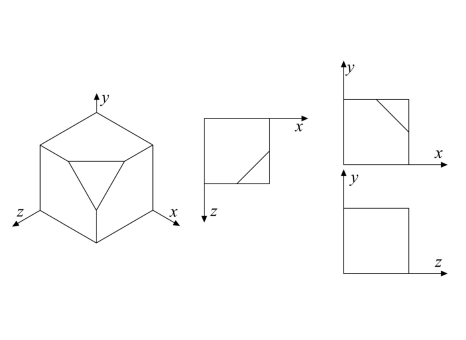
\includegraphics[width=0.5\textwidth]{images/ParOrth.png} 
    \caption{Prospective and Parallel}
    \label{fig:immagine}
\end{figure}
\subsubsection{Perspective projection matrix}
$M_{pro}=
\begin{bmatrix}
    1 & 0 & 0 & 0 \\
    0 & 1 & 0 & 0 \\
    0 & 0 & 1 & 0 \\
    0 & 0 & 1/d & 1 \\
\end{bmatrix}$
\\ \\ \\

$\frac{x_p}{d}=\frac{x}{z};
\frac{y_p}{d}=\frac{y}{z}, \\
x_p=\frac{x}{z/d}, y_p=\frac{y}{z/d}, z_p=d $\\
$ (x_p,y_p,z_p)=(\frac{x}{z/d},\frac{y}{z/d},d) $
$ M_{pro} *P=(X;Y;Z;W)=(x,y,z,\frac{z}{d}) $ \\
$(\frac{X}{W},\frac{Y}{W},\frac{Z}{W})=(x_p,y_p,z_p)=(\frac{x}{z/d},\frac{y}{z/d},d) $
\subsubsection{Parallel projection matrices}
\begin{figure}[H]
    \centering
    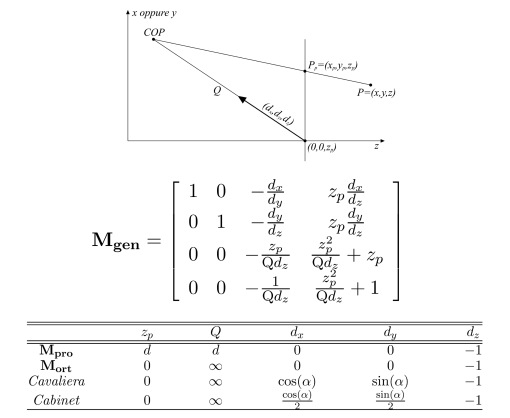
\includegraphics[width=0.5\textwidth]{images/ParPr.png} 
    \caption{Prospective projection matrix}
    \label{fig:immagine}
\end{figure}
$M_{ort}=
\begin{bmatrix}  
    1 & 0 & 0 & 0 \\
    0 & 1 & 0 & 0 \\
    0 & 0 & 0 & 0 \\
    0 & 0 & 0 & 1 \\
\end{bmatrix}$